\chapter{Introduction and What This Course Will Do for You and Your Purposes}

These notes follow Robert J. Shiller's opening lecture on financial markets, prepared for this series with curation by LazyingArt LLC. The lecture does not begin with trading rules, valuation formulas, or market lore. It begins by enlarging the meaning of finance. We are asked to see finance as one of the basic coordinating mechanisms of a modern society: it allocates resources across time, organizes risky ventures, rewards contribution, and makes large plans possible. From that opening point the lecture unfolds in a deliberate sequence: a broad philosophical claim, an insistence on institutional detail, a restrained but real mathematical preview, and finally a moral question about what finance is for.

\section{Finance as a Pillar of Civilized Society}

Shiller begins by taking the title \emph{Financial Markets} away from the narrow picture of trading and speculation. The word ``markets'' might suggest buying and selling securities, but the lecture immediately says that this is too small. Finance is presented instead as a pillar of civilized society. It is the structure through which large things are done.

\begin{definition}
In the sense of this lecture, finance is the set of institutions and arrangements through which society allocates scarce resources across time and uncertainty, sponsors collective ventures, incentivizes contribution, rewards constructive participation, and manages risk.
\end{definition}

The opening definition already carries a mathematical flavor, even though the lecture does not formalize it. If we want a minimal symbolic picture, we may think of a social plan as specifying a state-contingent allocation \(c_t(s)\), where \(t\) denotes time and \(s\) denotes a state of the world. Shiller does not develop a full equilibrium theory here, and we should not force one onto the lecture. The point is simpler and more foundational: finance concerns intertemporal and risky organization rather than mere exchange.

The lecture then identifies four functions that remain active throughout the course:

\begin{itemize}
\item allocation of resources across time and uncertainty,
\item incentive design,
\item sponsorship of ventures that require many participants,
\item management of uncertainty and risk.
\end{itemize}

Risk enters at once. Anything large or important that we do is uncertain. That is why financial markets matter. The opening claim is therefore not simply that finance moves money around. It is that finance lets us act under uncertainty without being paralyzed by uncertainty.

\begin{figure}[h]
\centering
\resizebox{0.92\linewidth}{!}{%
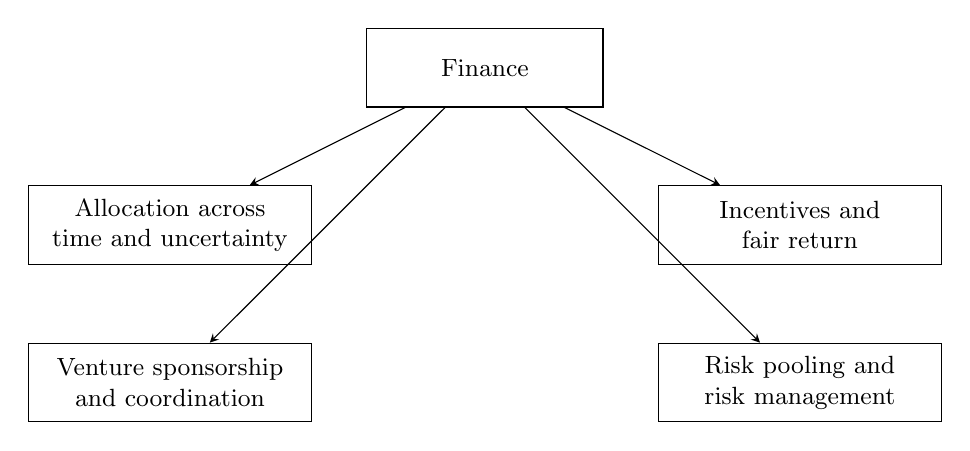
\begin{tikzpicture}[>=stealth, every node/.style={font=\small}]
\node[draw, rectangle, minimum width=3cm, minimum height=1cm, align=center] (f) at (0,0) {Finance};
\node[draw, rectangle, minimum width=3.6cm, minimum height=1cm, align=center] (a) at (-4,-2) {Allocation across\\time and uncertainty};
\node[draw, rectangle, minimum width=3.6cm, minimum height=1cm, align=center] (i) at (4,-2) {Incentives and\\fair return};
\node[draw, rectangle, minimum width=3.6cm, minimum height=1cm, align=center] (v) at (-4,-4) {Venture sponsorship\\and coordination};
\node[draw, rectangle, minimum width=3.6cm, minimum height=1cm, align=center] (r) at (4,-4) {Risk pooling and\\risk management};
\draw[->] (f) -- (a);
\draw[->] (f) -- (i);
\draw[->] (f) -- (v);
\draw[->] (f) -- (r);
\end{tikzpicture}%
}
\caption{Reconstruction of Shiller's opening picture of finance as a social technology.}
\end{figure}

That large opening claim is not left hanging. Shiller's next move is to say how such a subject must be studied.

\section{Philosophy, Detail, and a World Perspective}

Having made a broad civilizational claim, Shiller immediately narrows the method. The course will have a philosophical underpinning, but it will also be focused on details. This is one of the decisive sentences of the lecture. Finance is not to be discussed at the level of slogans. It is to be studied through institutions, contracts, and mechanisms, because, as he says, it is in the details that things happen.

The list of institutions arrives quickly: banking, insurance, securities, futures markets, derivatives markets, crises, and the future itself. The insistence on insurance is revealing. Some people treat insurance as if it were adjacent to finance rather than internal to it. The lecture refuses that separation. If finance is about risk-bearing and the organization of uncertain life, insurance belongs at the center.

The audience is then widened. The course has a U.S.\ bias because that is the institutional world Shiller knows best, but it is not meant to be provincially American. Many students will work outside the United States, and many listeners are not in the classroom at all. The Open Yale setting therefore matters intellectually, not just administratively. The lecture's international perspective is motivated twice over: by the future careers of the students, and by the fact that the course itself is being offered to the world.

This global orientation is reinforced by the historical moment. The course has been updated because finance changes quickly, and the recent financial crisis has forced governments around the world to reconsider regulation and institutional design. Shiller makes a sharp comparison here: an undergraduate physics course may need only modest updating over a few years, but finance cannot be treated that way. The crisis, the G20, and worldwide reform efforts are part of the subject itself.

The methodological principle is therefore clear. Large claims about finance must be tested and clarified at the level of institutions, and those institutions now operate in a global and rapidly changing setting. From there the lecture makes its next turn: if details matter, what role will mathematics play?

\section{Mathematics, Diversification, and the Real World}

Shiller places this course beside John Giannakopoulos's Econ 251. That other course is more theoretical and more mathematical. It includes state pricing, bond pricing, dynamic present value, uncertainty, hedging, the capital asset pricing model, and the leverage cycle. This course will not ignore mathematics, but it will use mathematics sparingly, intuitively, and always in the service of understanding the real world.

That restriction is not anti-mathematical. On the contrary, the lecture says mathematics is useful and cannot be avoided completely. Since many listeners will not take the more formal course, Shiller wants to provide the intuitive mathematical skeleton here. What he rejects is the idea that mathematics alone is the subject. The first mathematical spine of the course is already visible: independent risks, diversification, the law of large numbers, and the failure of the independence assumption in crisis.

\paragraph{Worked derivation.}
Let \(X_1,\ldots,X_n\) denote many separate risk exposures, and consider the equally weighted pooled exposure
\begin{equation}
\bar X_n=\frac{1}{n}\sum_{i=1}^n X_i.
\end{equation}
A direct variance calculation gives
\begin{align}
\operatorname{Var}(\bar X_n)
&=\operatorname{Var}\!\left(\frac{1}{n}\sum_{i=1}^n X_i\right) \\
&=\frac{1}{n^2}\sum_{i=1}^n \operatorname{Var}(X_i)
+\frac{2}{n^2}\sum_{i<j}\operatorname{Cov}(X_i,X_j).
\end{align}
If the risks are independent and each has variance \(\sigma^2\), then the covariance terms vanish and we obtain
\begin{equation}
\operatorname{Var}(\bar X_n)=\frac{\sigma^2}{n}.
\end{equation}
This is the simplest mathematical expression of the intuition Shiller emphasizes: if risks are independent, a large portfolio can diversify them away. In the same spirit, the law of large numbers may be written schematically as
\begin{equation}
\bar X_n \to \mathbb E[X]
\qquad \text{as } n\to\infty,
\end{equation}
which is just a formal way of saying that many independent fluctuations tend to average out.

At this point the lecture makes its crucial turn. The attractive theory becomes dangerous when it is trusted too much. The financial crisis is narrated as a failure of the independence assumption. Portfolio theory had encouraged people to think that perhaps one investment might go bad, but not all of them together. The crisis showed that this was false. In the language above, the neglected covariance terms return precisely in the bad states:
\begin{equation}
\begin{aligned}
\operatorname{Cov}(X_i,X_j) &>0 \quad \text{in crisis states} \\
&\Longrightarrow \text{losses do not average out.}
\end{aligned}
\end{equation}

This is all Shiller needs at this stage. He does not derive modern portfolio theory in full. He isolates its intuitive core, shows why it is attractive, and then shows why overconfidence in that core contributed to a worldwide crisis. The Great Depression enters here as the historical benchmark: by 1933 U.S.\ unemployment was about \(25\%\), and the recent crisis is presented as a near miss rather than a trivial disturbance.

An important philosophical point follows. The crisis does not, in Shiller's view, refute finance. Airplanes can crash without refuting aviation. Likewise, financial institutions can be fragile without ceasing to be socially indispensable. Once mathematics has been put into that proper place, the lecture can ask a more personal question: what is this course actually for?

\section{Why Everyone Needs Finance}

The lecture now shifts from method to purpose. Shiller's answer is strikingly broad: this is not merely a course for the subset of students who will enter the finance industry. Almost everyone should know finance, because finance is woven into the structure of ordinary and extraordinary life.

He even says, with some deliberate self-consciousness, that this may be one of the most useful courses in Yale College. That claim is not based on salaries alone. It is based on action. Finance prepares people to do things in the world. The lecture reinforces the point with a personal image: when Shiller gives talks on Wall Street, he likes to ask for a show of hands from former students who are now there. The anecdote is light in tone, but its function is serious. The course is meant to enter real careers and real institutions.

This is where the lecture raises a local tension. Is the course vocational? Shiller resists both extremes. It is not vocational in the vulgar sense of narrow job training. Yet it is also not detached from life. Yale may be a liberal-arts institution, but that does not mean it should disdain practical knowledge about how large things are actually done. He even jokes that perhaps a hermit does not need finance. Everyone else does.

The key analogy is memorable: finance is a kind of engineering, but it is an engineering that works with people rather than machines. That is why institutional detail matters. A course that refuses detail would be like a language course that refuses vocabulary. If we are to act in the world, we need to know the words of finance.

This is also why the lecture lingers over textbooks, readings, and concrete institutional categories. Shiller says he wants students to become interested in details, and he compares learning finance to learning a language with many thousands of words. The point is not pedantry. The point is that one cannot make things happen in a modern economy while remaining illiterate in its institutional grammar.

The lecture reinforces this with an occupational comparison reconstructed from a Bureau of Labor Statistics chart. Shiller emphasizes the projected 2018 bars because those are the careers his students are approaching. The point of the chart is not contempt for other fields. The point is relevance. Finance is not a tiny niche. It is a large and expanding zone of actual work and institutional responsibility.

\begin{table}[h]
\centering
\begingroup
\setlength{\tabcolsep}{3pt}
\small
\begin{tabular}{|p{0.50\linewidth}|p{0.18\linewidth}|}
\hline
Occupation mentioned in the lecture & Approx.\ magnitude \\
\hline
Financial analysts & \hfill \(300{,}000\) \\
Financial managers & \hfill \(>500{,}000\) \\
Personal financial advisors & \hfill \(250{,}000\) \\
Economists & \hfill \(20{,}000\) \\
\hline
\end{tabular}
\endgroup
\caption{Approximate occupational magnitudes cited in the lecture.}
\end{table}

The deeper point is larger than employment statistics. Finance should be understood as a general-purpose technology for action. If we want to organize households, firms, charities, cities, universities, or long-term projects, we cannot remain mystified by the financial language in which those things are arranged. That broad claim of usefulness now gives way to a harder question, because finance is also associated with great fortunes.

\section{Wealth, Scale, and Moral Purpose}

At this point the lecture introduces another text: Shiller's own unfinished manuscript, at that moment titled \emph{Finance and the Good Society}. He notes that the title may sound like an oxymoron. That is precisely the problem. Finance is under moral suspicion, especially after the crisis. People see bailouts, lobbying, and enormous private rewards. Why should this be thought of as a noble profession at all?

The Forbes 400 discussion is the lecture's answer-in-progress. It is not merely anecdotal color. It is the bridge from usefulness to moral tension. The point is that the richest people are typically not athletes or movie stars. Their wealth is usually tied to organizations, capital raising, ownership, acquisition, scaling, and deal-making. In other words, their power is institutional. They build and control arrangements through which many people work together.

This is why Shiller insists that finance is about making things happen on a large scale. It builds organizations. It marshals capital. It creates durable structures of coordination. The quiet people behind the scenes may matter more, in this institutional sense, than the visible celebrities.

The lecture then sharpens the question with arithmetic:
\begin{equation}
1\ \text{billion dollars}=1000\ \text{million dollars}.
\end{equation}
This elementary equality is used rhetorically, but it matters. Once one writes a billion dollars as a thousand million dollars, the ordinary consumer imagination begins to fail. One can buy cars and houses, but the scale quickly outruns ordinary consumption. The arithmetic forces the moral problem into view.

\subsection{Question \& Answer}

\paragraph{Question.}
What should immense financial success be for, once private consumption is no longer the real constraint?

\paragraph{Answer.}
The lecture answers this in stages. First, it rejects conspicuous consumption as an adequate answer. Sumptuary laws in many societies are cited as evidence that open display of wealth has long been felt to be socially suspect. The problem is not only envy. It is that mere display seems too small for fortunes of such magnitude.

Second, the lecture turns to Andrew Carnegie's \emph{Gospel of Wealth}. Carnegie's thesis is scandalous and interesting at the same time: those who are especially gifted at organizing business affairs have a moral obligation to redirect their fortunes toward public purposes rather than merely consume them or leave them to heirs. The fortune should not terminate in private luxury. It should be converted into institutions and public goods.

Shiller does not endorse this doctrine without qualification. He explicitly says there is only an element of truth in it. The strong claim that the rich are simply the most enlightened or deserving people is rejected. Yet the weaker claim is preserved: large-scale financial success becomes morally serious only when it is connected to purposes beyond personal display.

That is why Carnegie matters in the lecture. He is not introduced as a saint or as a theorem. He is introduced because he makes the problem vivid. If finance can create immense private wealth, then the moral question is what social form that wealth should eventually take. Carnegie's universities, halls, and public foundations are concrete answers, even if not a complete moral philosophy.

The lecture extends the same thought to the present, mentioning the campaign by Warren Buffett and Bill Gates to persuade billionaires to give most of their wealth away while still alive. At the same time, Shiller adds another qualification. There may even be a bubble in finance careers: as more people crowd toward a lucrative field, average outcomes may disappoint. Yet he still thinks that the top fortunes of the world will remain finance-related, precisely because the underlying technology scales so powerfully. The point is not that every financier is virtuous. The point is that finance, when it succeeds, creates a scale of action that immediately raises moral obligations.

From there the lecture moves back from moral philosophy into living institutions and living people.

\section{Finance in Action: Speakers, Regulation, and Behavioral Finance}

The outside speakers are not mere course logistics. They are embodiments of the lecture's thesis that finance is socially embedded and morally charged.

David Swensen is the clearest case. The lecture gives an explicit quantitative marker for the Yale endowment:
\begin{equation}
\begin{aligned}
E_{1985} &< \$1\text{ billion}, \\
E_{2008} &= \$22.9\text{ billion}, \\
E_{2010.06} &= \$16.7\text{ billion}.
\end{aligned}
\end{equation}
These numbers are used for more than admiration. They show the scale on which financial judgment can transform an institution. Swensen could have taken larger private compensation on Wall Street; the lecture presents his continued service at Yale as an example of finance directed toward a public purpose.

Maurice Hank Greenberg extends the point in a different register. Insurance, corporate power, philanthropy, and controversy are all brought together in one career. The lecture does not hide the scandal surrounding AIG, but it refuses to reduce Greenberg to the later collapse of a unit he no longer controlled. Again the pattern is the same: finance operates at a scale where institutional achievement and public scrutiny are inseparable.

Laura Cha supplies the missing regulatory pole. If finance involves incentives, risk, and the possibility of manipulation, then regulation is not external to finance. It is part of its moral and institutional architecture. The lecture is explicit on this point, and that is why a regulator belongs among the exemplary figures students are asked to hear.

The same expansion occurs in the teaching assistant discussion. Behavioral finance is introduced not as decorative psychology but as a change in how finance is understood. Mutual fund fee schedules, default choices, and consumer steering are cited as examples. A fund company may offer a menu of choices that looks benign on the surface but in practice steers clients toward arrangements that are not in their interest. This is exactly why finance cannot be treated as a purely mathematical subject. It is also about real people making choices under pressure, confusion, persuasion, competition, and imperfect information.

This movement from Swensen to Greenberg to Cha to behavioral finance completes a large arc of the lecture. Finance appears as portfolio management, insurance, regulation, and psychology all at once. Only now does Shiller open the subject into a full course roadmap.

\section{Preview of the Mathematical and Institutional Spine}

At the end of the lecture the outline of the course is given explicitly, but it no longer feels like administration. It feels like the consequence of everything that has already been argued.

\paragraph{Risk, crisis, and diversification.}
The next lectures begin with risk and financial crisis. Probability is mentioned, but only lightly. The mathematical core is exactly the one already isolated above: independent risks, diversification, law of large numbers, and the disaster that occurs when bad states produce common failure rather than cancellation. The capital asset pricing model is named as an important mathematical theory of diversification, but it is deferred rather than developed.

\paragraph{Technology, insurance, and efficient markets.}
Finance is then described as a technology. Securities, options, derivatives, and cash-flow partitions are treated as inventions rather than as arbitrary abstractions. Insurance becomes one of the central examples. It pools risk, prices uncertainty, and can improve safety by giving insurers an incentive to monitor the underlying environment. Efficient markets theory is previewed in the same restrained way: markets may often incorporate information rapidly, but the lecture refuses to turn that insight into a dogma.

\paragraph{Debt, equity, and contingent claims.}
Debt markets are introduced through the life cycle. A household may want a house before it has accumulated the cash to pay for one, so borrowing transfers purchasing power across time. Equity is introduced through a joint-enterprise example. Friends start a firm, but they contribute different amounts of capital, labor, and managerial effort. Shares are needed to divide claims and incentives:
\begin{equation}
\alpha_1+\alpha_2+\cdots+\alpha_m=1.
\end{equation}
This is not yet valuation theory. It is the simpler and more primitive problem of institutional design. The stock market, on this telling, is not primarily a casino. It is a mechanism for making collective enterprise stable and scalable. Options and other derivatives then appear as higher-order claims written on top of the underlying ownership structure.

\paragraph{Real estate, psychology, and banking.}
Real estate is flagged as both economically central and psychologically volatile. The recent crisis is linked to a bubble in home prices and to the collapse of that bubble. Behavioral finance will later return to the role of narratives, euphoria, and human judgment. Banking, multiple expansion of credit, and bank regulation are previewed as essential because the banking system itself nearly failed.

\paragraph{Later institutions.}
The remainder of the roadmap includes forwards and futures, options, monetary policy, investment banking, professional money management, exchanges, public finance, and nonprofit finance. The list is long, but the lecture's principle remains simple: each of these institutions is part of the machinery by which modern societies organize risk, capital, and purpose.

The final lecture of the course is said in advance to return to the question of purpose. This is the right ending because it is already the beginning. The entire roadmap is governed by the proposition that finance is not ultimately about making money. It is about giving shape to plans that would otherwise remain unrealized.

\section{Summary}

The first lecture does not yet teach a body of technical finance. It does something prior to that. It tells us what kind of subject finance is. It is a practical and moral technology of coordination under uncertainty. The mathematical content is real but deliberately modest: independence, averaging, diversification, and the failure of those ideas when correlations rise in crisis. Around that mathematical core the lecture builds a wider picture of institutions, incentives, regulation, wealth, philanthropy, psychology, and global change. The closing thought is therefore not an ornament. It is the governing thesis of the chapter: finance matters because it is one of the main ways in which we make our purposes happen.
